\documentclass{article}

%%%%%%%%%%%%%%% LIBRERIAS %%%%%%%%%%%%%%%%%%%%%
\usepackage{amsmath}
\usepackage{titlesec}
\usepackage{titletoc}
\usepackage{graphicx}
\usepackage[spanish,es-tabla]{babel} % 'es-tabla' cambia Cuadro→Tabla
\usepackage{hyperref}                % cargar después de babel
\usepackage{float}
\usepackage{circuitikz}
\usepackage[left=3cm,right=3cm]{geometry} %para margenes
%%%%%%%%%%%%%%%%%%% VARIABLES %%%%%%%%%%%%%%%%%%%%
\newcommand{\Facultad}{Instituto Tecnológico \\de\\ Buenos Aires} %constantes
\newcommand{\TPn}{Trabajo Práctico N° 3}
\newcommand{\TPtema}{Respuesta Transitoria}
\renewcommand{\thesection}{\arabic{section}}          % 2
\renewcommand{\thesubsection}{\quad \alph{subsection}}   % a
\renewcommand{\thesubsubsection}{\quad \thesubsection.~\roman{subsubsection}} % a. i
\graphicspath{{imagenes/}} %para que acceda a las fotos en la carpeta directamente


%%%%%%%%%%%%%%%%%% FORMATO TÍTULO Y NUMERACIÓN %%%%%%%%%%%%%%%%%%%
% Numeración de secciones
\renewcommand{\thesection}{\arabic{section}.}          
\renewcommand{\thesubsection}{\thesection\arabic{subsection}}       
\renewcommand{\thesubsubsection}{$\alph{subsubsection})$}

% Numerar hasta subsubsecciones
\setcounter{secnumdepth}{3}

% Formato de títulos
\titleformat{\section}{\Huge\bfseries}{\thesection}{1em}{}
\titleformat{\subsection}{\LARGE\bfseries}{\thesubsection}{0.5em}{}
\titleformat{\subsubsection}{\large\bfseries}{\thesubsubsection}{0.5em}{}



%%%%%%%%%%%%%%%%%%% ARCHIVO %%%%%%%%%%%%%%%%%%%%%%%%
\begin{document}

%%%CARATULA%%%
\begin{titlepage} %creo portada

        \begin{flushleft}
            \centering
            
\includegraphics[width=0.3\textwidth]{Logo_ITBA.png}
        \end{flushleft}

        \centering
            
        {\scshape\LARGE \Facultad \par} %\par sirve para indicar un final de parrafo
        \vspace{1cm}                    %esto hace un espacio entre lineas de 1cm


        {\huge\bfseries \TPn \par}
        \vspace{1.5cm}
        {\Large Teoría de Circuitos I\\ 25.10 \par}
        \vfill                      %sirve para rellenar el espacio y quede simétrico. Si se añaden otros, se dividen el espacio de forma equitativa
        {\Large \bfseries Grupo N° 2 \par}
        \vspace{1cm}
        {\large Juan Bautista Correa Uranga \hfill Legajo: 65016 \par} %\hfill sirve para hacerlo simétrico
        {\large Juan Ignacio Caorsi \hfill Legajo: 65532  \par}
        {\large Rita Moschini \hfill Legajo: 67026 \par} 
        \vfill
        {\large \today\par}
        \vfil

    \end{titlepage}

 %%%RESUMEN%%%
{\centering \LARGE \bfseries Resumen \par}

\newpage

%%%INDICE%%%
\tableofcontents %esto sirve para crear el índice

\newpage

%%%Introduccion%%%
\section{Introducción}
    Este trabajo práctico aborda la respuesta transitoria
     en circuitos RLC serie. Se busca aplicar conceptos 
     teóricos mediante mediciones reales, utilizando generador 
     de señales y osciloscopio. Se analiza cómo varían las
      respuestas al modificar resistencia, inductancia y 
      capacitancia, observando casos de subamortiguamiento,
       sobreamortiguamiento y amortiguamiento crítico. 
       El objetivo es comprender la dinámica temporal 
       de circuitos RLC y validar modelos teóricos
       con datos experimentales.
    \subsection{Instrumental}
        En esta experiencia se utilizaron los siguientes instrumentos:
\begin{itemize}
  \item Osciloscopio Keysight DSOX 1202G con generador de ondas integrado.
  \item Capacitores de $47\,\text{pF}$ y $470\,\text{pF}$.
  \item Resistencias de 220 $\Omega$ nominal y potenciómetro de 5 k$\Omega$ nominal.
  \item Inductor de resistencia indefinida, con inductancia aproximada de $1\,\text{mH}$.
  \item Multímetro UNI-T,  Standar Digital multimeter, modelo: UT39C.
\end{itemize}

    \subsection{Marco teórico}

        Un circuito RLC serie está compuesto por una resistencia (R),
         una 
        inductancia (L) y una capacitancia (C) conectadas en serie.
        Dependiendo de la resistencia del circuito, la respuesta transitoria
         puede ser subamortiguada, sobreamortiguada o críticamente 
         amortiguada. La ecuación diferencial que describe la 
         respuesta del circuito RLC serie es:
        \begin{equation}
            L\frac{d^2i(t)}{dt^2} + R\frac{di(t)}{dt} + \frac{1}{C}i(t) = V_{in}(t)
        \end{equation}

        y su solución general es la suma de la respuesta natural y la respuesta forzada:

Para la respuesta natural (\( V_{\text{in}}(t) = 0 \)), se define:

\begin{equation}
\alpha = \frac{R}{2L}, \quad \omega_0 = \frac{1}{\sqrt{LC}}, \quad \Delta = \alpha^2 - \omega_0^2
\end{equation}

La solución general depende del valor de \( \Delta \):

\begin{itemize}
  \item \textbf{Sobreamortiguado} (\( \Delta > 0 \)):

  \begin{equation}
  i(t) = A e^{(-\alpha + \sqrt{\Delta})t} + B e^{(-\alpha - \sqrt{\Delta})t}
  \end{equation}

  \item \textbf{Críticamente amortiguado} (\( \Delta = 0 \)):

  \begin{equation}
  i(t) = (A + Bt)e^{-\alpha t}
  \end{equation}

  \item \textbf{Subamortiguado} (\( \Delta < 0 \)):

  \begin{equation}
  i(t) = e^{-\alpha t} \left( A \cos(\omega_d t) + B \sin(\omega_d t) \right)
  \end{equation}

  donde \( \omega_d = \sqrt{\omega_0^2 - \alpha^2} \).
\end{itemize}

%%%Desarrollo%%%
\section{Desarrollo}
    \subsection{Procedimiento}

\begin{figure}[H]
    \centering
    \begin{tikzpicture}
        \draw (15.75, -14.5) to[american voltage source, l={$Vs$}] (15.75, -17.75);
        \draw (15.75, -14.5) to[american resistor, l={$Rf$}] (19.5, -14.5);
        \draw (19.5, -14.5) to[variable american resistor, l={$Rv$}] (22.25, -14.5);
        \draw (22.25, -14.5) to[cute inductor, l={$L$}] (22.25, -17.75);
        \draw (22.25, -17.75) to[capacitor, l={$C$}] (15.75, -17.75);
    \end{tikzpicture}
    \caption{Circuito analizado}
    \label{fig: circuito_rlc}
\end{figure}


    La parte experimental se realizó en una serie de 4 pasos:

    \begin{enumerate}
        \item Primero se armó el circuito en serie (observar figura \ref{fig: circuito_rlc}) usando el capacitor de 470 pF. Luego, se determinó de manera aproximada, observando la salida en el osciloscopio, el valor de la resistencia variable que producía un amortiguamiento crítico.
        \item En esta parte, se ajustó la resistencia Rv a su valor máximo. Poteriormente, se coloco uno de los cursores horizontales del osciloscopio en $ V_{salida}=0 V$, y el otro en $ V_{salida}=3,16 V$ y medimos el $ \Delta t $ entre esos valores, tomandolo como el $\tau$ del sistema. Con este valor aproximado, se midió la salida en el tiempo $ 5\tau$.
        \item A continuación, se remplazo el capacitor por uno de 47pF, y se repitió la medición de la resistencia variable tal que el amortiguamiento fuera crítico. Luego, se puso Rv en su valor mínimo, y se calculó el tiempo del transitorio. También se midió la frecuencia y el valor de sobrepico, esto el $ \Delta V = V_{max} - V_{excitacion} = V_{max} - 5 V $. Para calcular la frecuencia, obtuvimos un valor aproximado del periodo promediando las distancias horizontales entre los primeros 3 picos.
        \item Finalmente, se cortocircuitaron las resistencias y se analizó el tiempo de respuesta transitoria nuevamente.
        
    \end{enumerate}
    \subsection{Mediciones}
 
        \begin{itemize}
            \item $ R_f = 215 \Omega $
            \item $ R_{V_{max}} = 9980 \Omega $
            \item $ R_{V_{min}} = 2 \Omega $
            \item $ R_L = 0,8 \Omega $
            \item $ L \approx 1 mH $
        \end{itemize}
        
        \par
        \subsubsection*{Capacitor de C = 470 pF}
            \begin{itemize}
                \item Resistencia variable tal que el amortiguamiento fue crítico: $ R_{critico} = 1,9 k\Omega $ % item 1
                \item Tiempo $\tau$ en que la salida llegó a 3,175 V con $ R_V $ en su valor máximo: $ \tau = 5,75 \mu s$ % item 2
                \item Salida cuando $t=5\tau$ con $ R_V $ en su valor máximo: $V_{5\tau}$ = 5 V% item 2
            \end{itemize}

        \par
        \subsubsection*{Capacitor de C = 47 pF}
            \begin{itemize}
                \item Resistencia variable tal que el amortiguamiento fue crítico: $ R_{critico} = 3,47 k\Omega $ %item 3
                \item Tiempo en que la salida llegó a 3,175 V con $ R_V $ en su valor crítico: $ t = 2,20 \mu s$ % item 3
                \item Tiempo en que la salida llegó a 5,24 V con $ R_V $ en su valor mínimo: $ t = 14,30 \mu s$ % item 4
                \item Tiempo en que la salida llegó a 4,982 V ($ 5V \pm 0,05V $) con las resistencias cortocircuitadas: $ t = 11 \mu s$ % item 5
            \end{itemize}

    \subsection{Cálculos}

        \subsubsection{Ecuaciones utilizadas}            

            \textbf{Cálculo del la resistencia variable tal que el amortiguamiento fuera crítico} \par \par
            $ \alpha_{serie} = \omega_0 \Rightarrow \frac{R}{2L} = \frac{1}{\sqrt{LC}}  $
            \begin{equation}
                R = \frac{2L}{\sqrt{LC}}
            \end{equation}  \par \par 

            \textbf{Cálculo de la inductancia} \par \par
            Tomando la resistencia variable tal que el amortiguamiento resultase crítico,
            $ R = \frac{2L}{\sqrt{LC}} = 2\frac{\sqrt{L}}{\sqrt{C}} $
            \begin{equation}
                L = \frac{C \cdot R^2}{4}
            \end{equation}

            
        \subsubsection{Resultados}

            \subsubsection*{Capacitor de C = 470 pF}
                0) Inductancia L
                \begin{equation}
                    L=0.526mH
                \end{equation}
                1) Resistencia variable tal que el amortiguamiento fuera crítico:
                \begin{equation}
                    R_{critico} = 1.857 k\Omega
                \end{equation} \par
                2) $ \tau $ con $ R_V = R_{V_{max}} = 9980 \Omega $:
                 \begin{equation}
                    \tau = 4,74 \mu s 
                \end{equation}

            \subsubsection*{Capacitor de C = 47 pF}
                3) Resistencia variable tal que el amortiguamiento fuera crítico:
                \begin{equation}
                    R_{critico} = 6,47 k\Omega 
                \end{equation} \par
                4) Valor de $ \tau $ para $ R_V = R_{V_{min}} $: 
                \begin{equation}
                    \tau = 4,83 \mu s 
                \end{equation} \par
                6) Valor de $ \tau $ para $ R = R_L $ (resistencias cortocircuitadas): REVISAR
                \begin{equation}
                    \tau =  1,315 ms 
                \end{equation}
        


    \subsection{Análisis}
    
    	Luego de recolectar los datos, se pudieron observar los siguientes comportamientos. \par
	Es importante mencionar que en este trabajo, no se contó con un valor de referencia de la constante del inductor; esta debió ser aproximada mediante el valor de la resistencia del amortiguamiento crítico obtenida con el capacitor de 470 pF. Consecuentemente, los datos teóricos también pueden contener errores asociados.
	
        \subsection*{Capacitor 470 pF}
        	En esta parte, se observó lo siguiente: al aproximar el valor de la resistencia del amortiguamiento crítico, se llegó a $1,9 k\Omega$, un valor el cual posee un error relativo del 2,32 \% con respecto al valor teórico. Esto indica una buena aproximación al valor real que causa que el sistema sea críticamente amortiguado. \par
	Sumado a esto, se observó que la respuesta se volvía sobreamortiguada al aumentar la resistencia por encima de $1,9 k\Omega$ y que la misma se volvía subamortiguada al disminuir la misma por debajo de ese valor. Esto concuerda con las ecuaciones descriptas en el apartado teórico, puesto a que al aumentar R, $\alpha$ aumentaba. \par
	Otras de las áreas analizadas fue la del valor de $\tau$. Esta se aproximó despejando el tiempo el cual llevaba a una respuesta de 3,175 $V$. Se observó que el mismo fue de $5,75 \mu F$, un valor el cual posee un error relativo del 21,3\%. Esto muestra un error alto, pero el mismo puede estar asociado en gran medida a la incertidumbre en el valor de la constante L. Al mismo tiempo, dicho $\tau$ teórico se consiguió mediante una aproximación, usando la raíz de la ecuación característica más pequeña y descartando la otra.\par
	Finalmente, se observó que el transitorio en $5\tau$ el valor de la respuesta estaba entre los valores de 4,75 V y 5,25 V. Esto demuestra que la aproximación de $5\tau$ como tiempo de transitorio, es efectiva.
	
	
        \subsection*{Capacitor 47 pF}
        En esta parte, se analizó el efecto de la reducción de la capacitancia. Primero se observo que la resistencia del valor crítico aumentaba en comparación con el capacitor de 470 pF. Consecuentemente, esto aumentó el margen de valores de las resistencias en los cuales el sistema se mantiene como un subamortiguado.\par
        Al mismo tiempo, también se midió un valor de resistencia que causaba un amortiguamiento crítico. Ese valor fue de $3,47 k\Omega$, el cual muestra un error relativo del 46,4\%. Este gran error asociado a la medición se debe a que el valor fue obtenido de manera aproximada, sin un ajuste riguroso.\par 
        
        \begin{figure}[h!]
    \centering
    \begin{minipage}{0.49\textwidth}
        \centering
        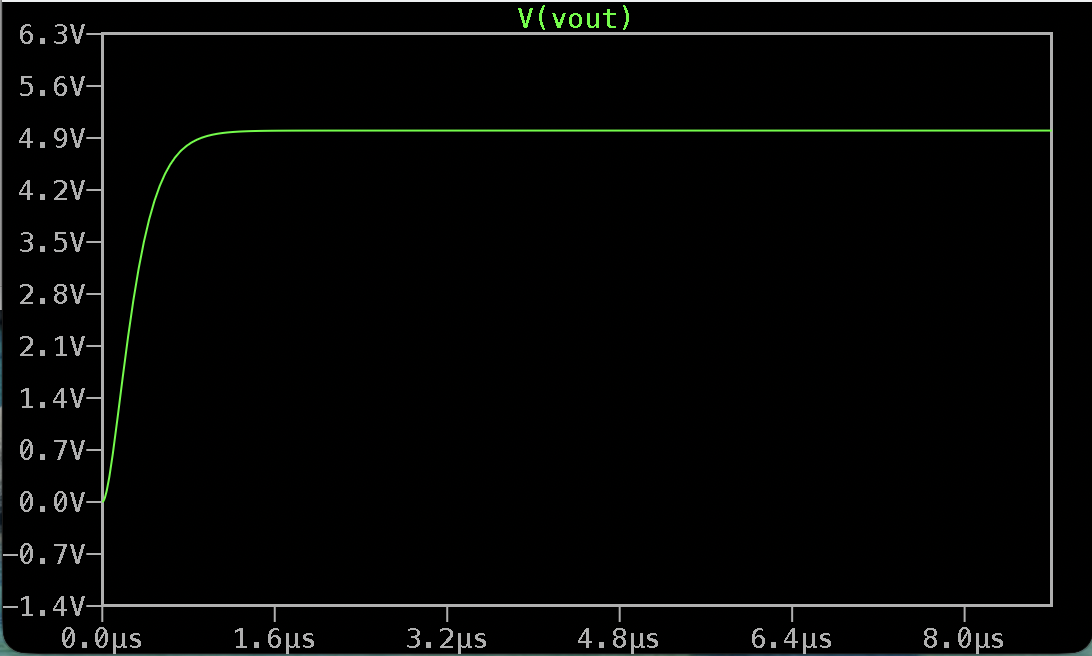
\includegraphics[width=\linewidth]{CRIT2.png}
        \caption{Capacitor 47pF, con Rv = 6,47 $k\Omega$}
        \label{fig:img1}
    \end{minipage}\hfill
    \begin{minipage}{0.49\textwidth}
        \centering
        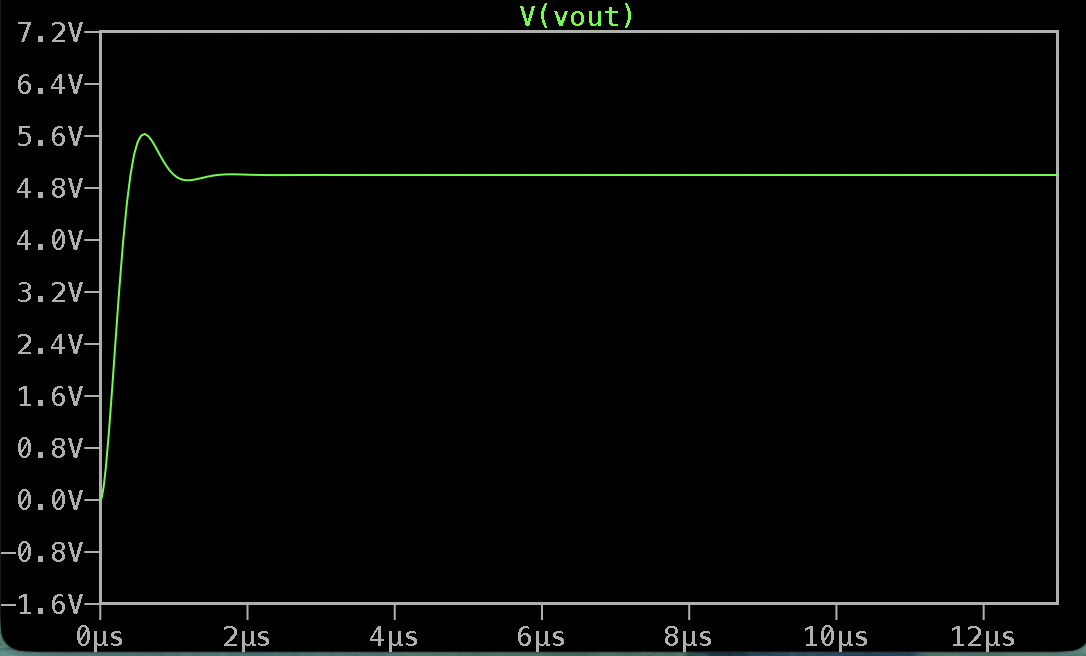
\includegraphics[width=\linewidth]{SUBAMORT1.png}
        \caption{Capacitor 47pF, con Rv= 3,47 $k\Omega$}
        \label{fig:img2}
    \end{minipage}
\end{figure}

        Por este motivo, se recurrió a la simulación del mismo usando el valor de L. Es importante volver a mencionar que el mismo ya asocia una gran incertidumbre en su cálculo. Al observar las figuras \ref{fig:img1} y \ref{fig:img2}, se puede observar que el valor calculado mediante el osciloscopio, es un valor subamortiguado. Por tal motivo se considera que el valor de 6,47 $k\Omega$ es el valor aproximado que genera un transitorio críticamente amortiguado.\par
        Por otra parte, al analizar el tiempo de transitorio del sistema, con la resistencia variable configurada en su valor mínimo, se obtuvieron los datos a continuación. El tiempo de respuesta transitoria obtenido experimentalmente fue de 14,30 $\mu$s, un valor muy lejano al que se consigue con la aproximación teórica de $5\tau$ = 24,15 $\mu$s. \par
        
        
                \begin{figure}[h!]
    \centering
    \begin{minipage}{0.49\textwidth}
        \centering
        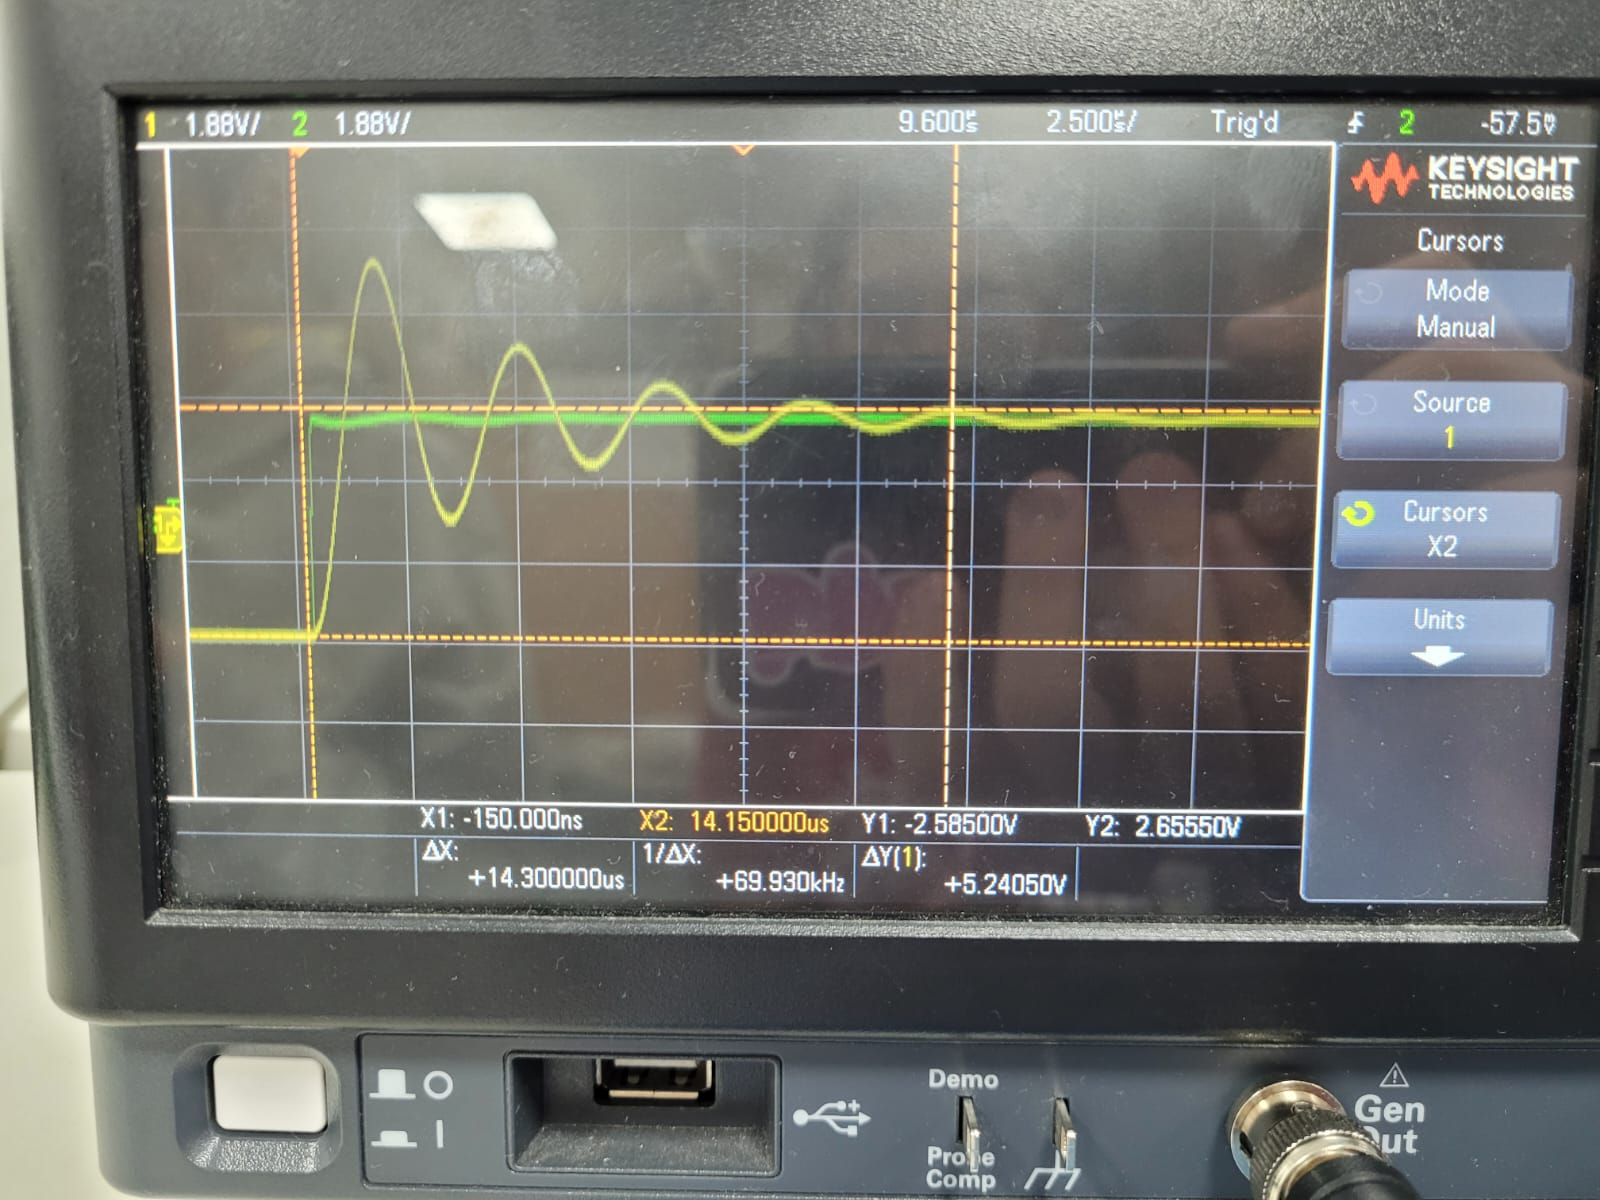
\includegraphics[width=\linewidth]{OSI5T.jpg}
        \caption{Foto de medición de 5tau con la resistencia mínima.}
        \label{fig:taureal}
    \end{minipage}\hfill
    \begin{minipage}{0.49\textwidth}
    \centering
 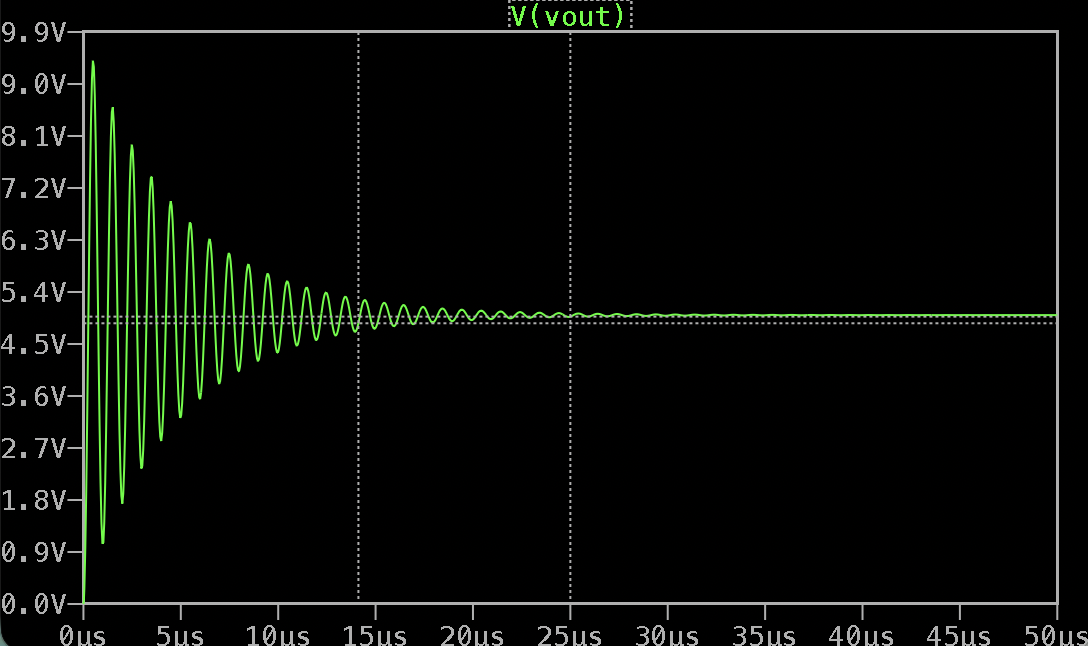
\includegraphics[width=\linewidth]{TAU47PF.png}
        \caption{Capacitor 47pF, con Rv mínimo. Aquí la linea marca el valor de 5$\tau$. }
        \label{fig:tausim}

    \end{minipage}
\end{figure}

   
  Al observar las dos gráficas (observar figuras \ref{fig:taureal} y \ref{fig:tausim}), se puede observar que el gráfico teórico difiere en gran medida con el medido por el osciloscopio. Las dos diferencias más grandes que se observa son: 1) La señal medida por el osciloscopio posee un decaimiento exponencial mucho más rápido que la simulada. 2) La señal simulada posee una frecuencia angular mucho más rápida que la medida por el osciloscopio. \par 
  Esta gran diferencia se puede explicar por el efecto de histéresis en el inductor. Si bien el núcleo del inductor es de ferrite, un material el cual no cuenta con perdidas a causa de corrientes Eddin, el mismo cuenta con perdidas de histéresis al cambiar la orientación del campo magnético. Esto se debe a que la corriente en este momento no es continua, sino que varia con el tiempo cambiando la dirección del campo magnético. Esto termina afectando la energía del sistema no ideal, causando las diferencias observadas con los valores teóricos.\par
  Por tal motivo, se pudo concluir que en este caso los cálculos teóricos no se aproximan correctamente a los valores observados en el sistema real. Esto se debe a que las ecuaciones no contemplan el efecto de perdida causado por la histéresis. Es más, este modelo se podría aproximar usando una resistencia en serie o una resistencia en paralelo. Aunque la misma conserva una forma parecida, la misma cuenta con diferencias marcadas en el tiempo de transitorio, por lo que no se consideró pertinente su comparación con los valores experimentales. Todo esto explicaría el error relativo del 68\% entre el tiempo del transitorio teórico y el experimental.\par
  (explicar sobre pico)\par
  En última instancia se cortocircuitaron la resistencia de 215 $\Omega$ y la resistencia variable. Al comparar ambos gráficos (observar figuras \ref{fig:CORTREAL} y \ref{fig:CORTSIM}), se puede observar una gran diferencia entre los datos obtenidos teóricamente y los datos empíricos. Mientras que según lo teórico se puede observar lo que es un oscilador casi ideal, en la experiencia de laboratorio se observo un sistema que no oscila indefinidamente. Esto se puede ver en los datos, puesto a que el tiempo de transitorio obtenido en el osciloscopio es de $ t = 11 \mu s$, mientras que el teórico es de $5\tau$ = 6,58 ms. Esto es una diferencia de 3 ordenes de magnitud.\par
  Esta diferencia vuelve a ser explicada por la perdida de histéresis en el inductor. En el modelo teórico se considera que el único elemento que pierde energía es la resistencia asociada al inductor. No obstante en la realidad, el sistema no solo pierde energía por la resistencia del inductor, sino que también por la histéresis al cambiar la orientación del campo magnético.
  
                  \begin{figure}[h!]
    \centering
    \begin{minipage}{0.49\textwidth}
        \centering
        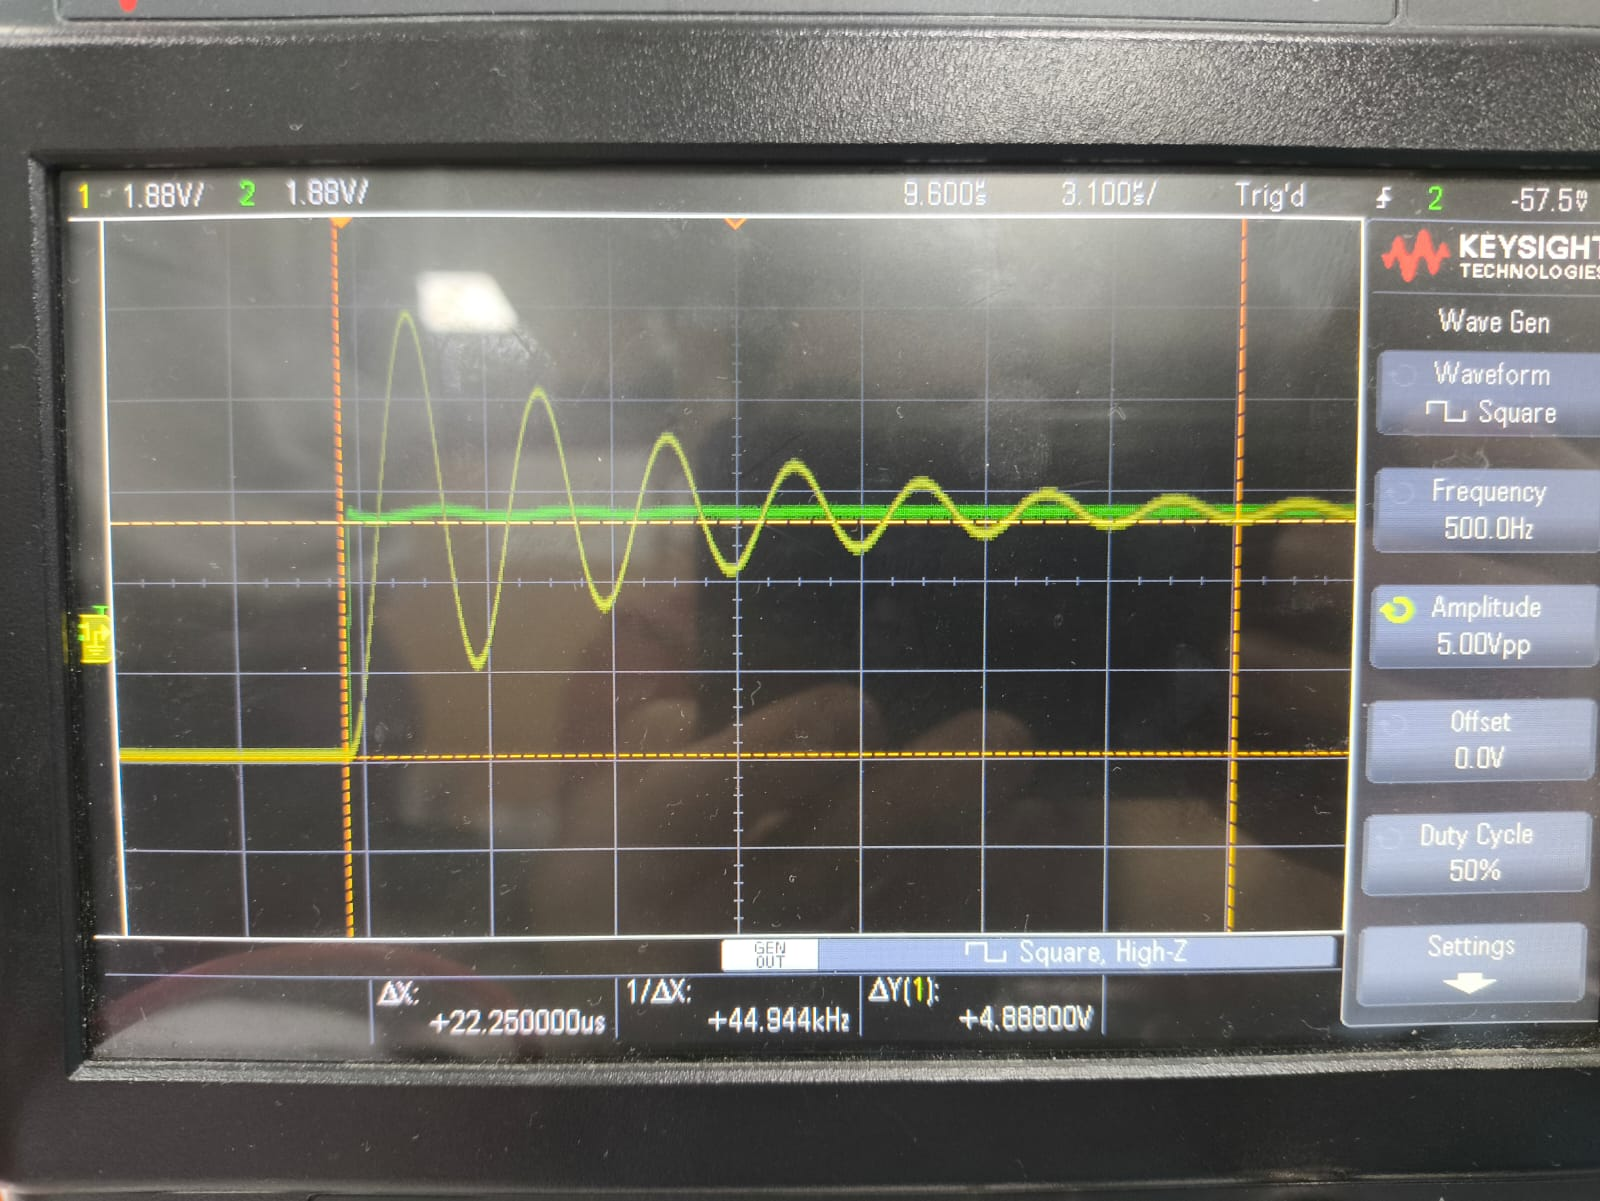
\includegraphics[width=\linewidth]{Resistencias_corto.jpg}
        \caption{Foto de medición del osciloscopio con las resistencias cortocircuitadas.}
        \label{fig:CORTREAL}
    \end{minipage}\hfill
    \begin{minipage}{0.49\textwidth}
    \centering
 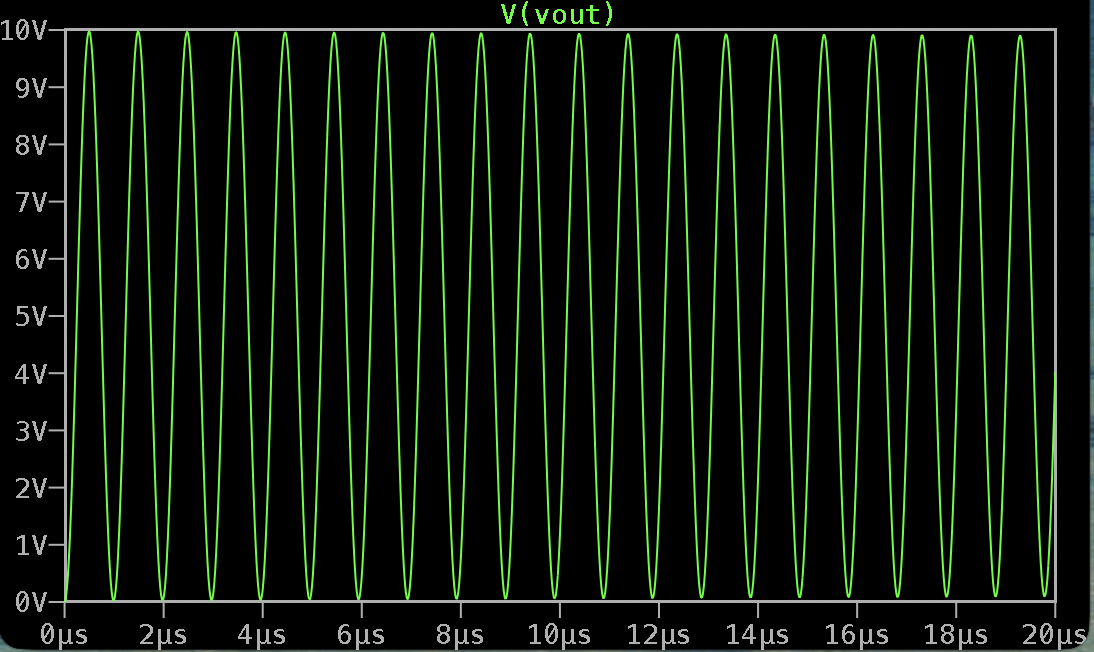
\includegraphics[width=\linewidth]{CORTOCIRCUITO.png}
        \caption{Simulación del sistema con las resistencias cortocircuitadas. }
        \label{fig:CORTSIM}

    \end{minipage}
\end{figure}

  
  
  
 
    
    
    
   
   
        
        

\subsection*{Rita}
Procedimiento
- la oracion "luego de esto, se observo la rta del sist en funcion del valor de la resistencia variable' me parece que no aporta.


Analisis
- no me convence la justifiacion de que el tau con C=470pF tiene mucho error por culpa del L. Con ese criterio, todo lo calculado con ese L deberia tener mucho error
- con C=47pF esta puesto que al reducirse la capacitancia, el valor de R critico aumenta, pero no se justifica por que
- en la justificacion de por que la resistencia del critico tiene casi 50 \% de error esta puesto que es xq se obtuvo de manera aproxmada, sin un ajuste riguroso. Tendría que esta aclarado como se obtuvo, que es esa "manera aproximada"



\section{Conclusiones}

\end{document}